% !TEX root = ../main.tex
\setchapterimage{figure/C2封面图.png}
\setchapterintro{}
\chapter{子群}
\section{定义与例子}
\begin{definition}
	 设 $G$ 是一个群。若 $G$ 的子集 $H$ 非空，并且对乘积和取逆封闭（即 $x,y\in H$ 蕴含 $x^{-1}\in H$ 且 $xy\in H$），则称 $H$ 是 $G$ 的一个\textbf{子群}。若 $H$ 是 $G$ 的子群，记作 $H\leqslant G$。
\end{definition}



当我们说 $H$ 是 $G$ 的子群时，总是指 $H$ 上的群运算是 $G$ 上的运算限制到 $H$ 得到的运算。正如我们对函数限制到子集时所做的那样，我们用同一个符号表示 $G$ 的运算和子群 $H$ 的运算。若 $H\leq G$ 且 $H\neq G$，则写作 $H<G$，以强调包含是真包含。

若 $H$ 是 $G$ 的子群，则由于 $H$ 的运算是 $G$ 的运算在 $H$ 上的限制，$H$ 中的任何等式也可看作 $G$ 中的等式。因此，$G$ 中的消去律说明：$H$ 的单位元与 $G$ 的单位元相同（特别地，每个子群都必须含有 $1$，即 $G$ 的单位元）；并且 $H$ 中元素 $x$ 的逆元，与把 $x$ 看作 $G$ 中元素时的逆元相同。

\begin{example}
	\begin{enumerate}[label=(\arabic*)]
		\item 在加法运算下，$\ZZ\leq \QQ$ 且 $\QQ\leq \RR$。
		\item 任意群 $G$ 都有两个子群：$H=G$ 和 $H=\{1\}$；后者称为\textbf{平凡子群}，今后记作 $1$。
		\item “是……的子群”这一关系具有传递性：若 $H$ 是群 $G$ 的子群，$K$ 是 $H$ 的子群，则 $K$ 也是 $G$ 的子群。
	\end{enumerate}
\end{example}

\begin{proposition}
	（子群判别法） 群 $G$ 的子集 $H$ 是子群，当且仅当
\begin{enumerate}[label=(\arabic*)]
	\item $H\neq\varnothing$；
	\item 对所有 $x,y\in H$，$xy^{-1}\in H$。
\end{enumerate}
此外，若 $H$ 是有限集，则只需检查 $H$ 非空且对乘法封闭。
\end{proposition}
\begin{proof}
	必要性：若 $H$ 是 $G$ 的子群，则 (1) 和 (2) 显然成立，因为 $H$ 含有 $G$ 的单位元、含有每个元素的逆元，并且对乘法封闭。
	
	充分性：假设 $H$ 满足 (1) 和 (2)，我们证明 $H\leq G$。
	
	取 $H$ 中任意元素 $x$。令 $y=x$ 并应用 (2)，得 $1=xx^{-1}\in H$，所以 $H$ 含有 $G$ 的单位元。
	
	再由 (2)，由于 $H$ 含有 $1$ 和 $x$，$H$ 含有元素 $1x^{-1}$，即 $x^{-1}\in H$，所以 $H$ 对取逆封闭。
	
	最后，若 $x,y$ 是 $H$ 的任意两个元素，则由刚才证明，$y^{-1}\in H$；再由 (2)，$H$ 也含有 $x(y^{-1})^{-1}=xy$。因此 $H$ 也对乘法封闭，从而 $H$ 是 $G$ 的子群。
	
	现在假设 $H$ 有限且对乘法封闭，取任意 $x\in H$。在 $x,x^2,x^3,\ldots$ 中只有有限多个不同元素，所以存在整数 $a,b$，$b>a$，使得 $x^a=x^b$。若 $n=b-a$，则 $x^n=1$，因此 $H$ 中每个元素都有有限阶。于是 $x^{n-1}=x^{-1}$ 属于 $H$，所以 $H$ 自动对取逆封闭。
\end{proof}
\section{中心化子与正规化子，稳定子与核}
\begin{definition}
	定义
	\[
	C_G(A)=\{g\in G\mid gag^{-1}=a\text{ 对所有 }a\in A\}.
	\]
	这个 $G$ 的子集称为 $A$ 在 $G$ 中的\textbf{中心化子}。由于 $gag^{-1}=a$ 当且仅当 $ga=ag$，$C_G(A)$ 就是 $G$ 中与 $A$ 的每个元素都交换的那些元素组成的集合。
\end{definition}
利用子群判别法，可以证明$C_G(A)$是$G$的子群.
\begin{proposition}
	$C_G(A)$是$G$的子群.
\end{proposition}
\begin{proof}
	显然 ，$e\in C_G(A)$,那么$\forall x,y\in C_G(A)$,考虑$xy^{-1}$,任取$a\in A $,由 $x,y\in C_G(A)$，有$xax^{-1} = a ,yay^{-1} = a \iff y^{-1}a y = a$
	\[(xy^{-1})a(xy^{-1})^{-1}  = xy^{-1}a y x^{-1} = x(y^{-1}a y )x^{-1} = xax^{-1} =a\]
	从而$xy^{-1}\in  C_G(A)$,故$ C_G(A)\leqslant G$
\end{proof}

在特殊情形 $A=\{a\}$ 下，我们简写 $C_G(a)$ 而不是 $C_G(\{a\})$。此时对所有 $n\in\ZZ$，都有 $a^n\in C_G(a)$。

\begin{definition}
	定义
	\[
	Z(G)=\{g\in G\mid gx=xg\text{ 对所有 }x\in G\},
	\]
	即与 $G$ 中所有元素都交换的元素集合。这个 $G$ 的子集称为 $G$ 的\textbf{中心}。
\end{definition}
注意 $Z(G)=C_G(G)$，所以上面的证明把 $Z(G)\leq G$ 作为特殊情形证明了.

\begin{definition}
	定义
\[
gAg^{-1}=\{gag^{-1}\mid a\in A\}.
\]
定义 $A$ 在 $G$ 中的\textbf{正规化子}为
\[
N_G(A)=\{g\in G\mid gAg^{-1}=A\}.
\]
\end{definition}
容易证明
\[C_G(A)\leqslant N_G(A)\leqslant G \]


\begin{definition}
	若群 $G$ 作用在集合 $S$ 上，且 $s$ 是 $S$ 中的某个固定元素，则 $s$ 在 $G$ 中的\textbf{稳定子}是集合
\[
G_s=\{g\in G\mid g\cdot s=s\}
\]
\end{definition}
\begin{proposition}
\[ 	G_s\leqslant G \]
\end{proposition}
\begin{proof}
	显然$1 \in G_s,$任取$x,y \in G_s $
	\begin{align*}
		s &= 1\cdot s=(y^{-1}y)\cdot s\\
		&= y^{-1}\cdot (y\cdot s) &&\text{（由作用公理 (1)）}\\
		&= y^{-1}\cdot s &&\text{（因为 $y\in G_s$），}
	\end{align*}
	那么
	\[xy^{-1}\cdot s= x\cdot s = s\]
	
\end{proof}
类似的，我们定义出$G$在$S$上作用的核，定义为
\begin{definition}
	$G$在$S$上作用的核定义为 
	\[\ker G = \{ g\in G : g\cdot s =s \text{对所有的}s\in S\}\]
\end{definition}
并且利用子群判别法，容易证明$\ker G \leqslant G$

\section{循环群与循环子群}


\begin{definition}
	 群 $H$ 称为\textbf{循环的}，如果 $H$ 可由单个元素生成；也就是说，存在某个 $x\in H$，使得
	\[
	H=\{x^n\mid n\in\ZZ\}
	\]
	记作$H=\langle x\rangle$，并称 $H$ 由 $x$ 生成（$x$ 是 $H$ 的生成元）
\end{definition}

一个循环群可以有不止一个生成元。例如，若 $H=\langle x\rangle$，则也有 $H=\langle x^{-1}\rangle$，因为 $(x^{-1})^n=x^{-n}$，而当 $n$ 遍历所有整数时，$-n$ 也遍历所有整数，所以
\[
\{x^n\mid n\in\ZZ\}=\{(x^{-1})^n\mid n\in\ZZ\}.
\]
由指数律，循环群都是阿贝尔群。
\begin{example}
	设 $G=D_{2n}=\langle r,s\mid r^n=s^2=1,
	rs=sr^{-1}\rangle$，$n\geq 3$，并令 $H$ 为正 $n$ 边形所有旋转构成的子群。因此 $H=\langle r\rangle$，且 $H$ 的不同元素为
	\[
	1,r,r^2,\ldots,r^{n-1}
	\]
	（这些是 $r$ 的所有不同幂）。特别地，$|H|=n$，$H$ 的生成元 $r$ 的阶为 $n$。$r$ 的幂以周期 $n$“循环”（向前或向后），即
	\[
	r^n=1,
	\quad r^{n+1}=r,
	\quad r^{n+2}=r^2,\ldots,
	\]
	且
	\[
	r^{-1}=r^{n-1},\quad r^{-2}=r^{n-2},\ldots
	\]
	一般地，要把任意幂 $r^t$ 写成 $r^k$，其中 $0\leq k<n$，用除法算法写
	\[
	t=nq+k,
	\qquad 0\leq k<n,
	\]
	则
	\[
	r^t=r^{nq+k}=(r^n)^q r^k=1^q r^k=r^k.
	\]
\end{example}
\begin{proposition}\label{循环群的阶数}
	若 $H=\langle x\rangle$，则 $|H|=|x|$（若等式一边为无穷，则另一边也为无穷）。更具体地：
	\begin{enumerate}[label=(\arabic*)]
		\item 若 $|H|=n<\infty$，则 $x^n=1$，且 $1,x,x^2,\ldots,x^{n-1}$ 是 $H$ 的全部不同元素；
		\item 若 $|H|=\infty$，则对所有 $n\neq 0$ 有 $x^n\neq 1$，且对 $\ZZ$ 中不同的 $a,b$ 有 $x^a\neq x^b$。
	\end{enumerate}
	
\end{proposition}
\begin{proof}
	设 $|x|=n$。先考虑 $n<\infty$ 的情形。元素 $1,x,x^2,\ldots,x^{n-1}$ 彼此不同，因为若 $x^a=x^b$，不妨设 $0\leq a<b<n$，则 $x^{b-a}=x^0=1$，这与 $n$ 是使 $x$ 的正幂等于单位元的最小正整数矛盾。因此 $H$ 至少有 $n$ 个元素，还需说明这些就是全部元素。若 $x^t$ 是 $x$ 的任意幂，用带余除法写 $t=nq+k$，其中 $0\leq k<n$，于是
	\[
	x^t=x^{nq+k}=(x^n)^qx^k=1^qx^k=x^k\in\{1,x,x^2,\ldots,x^{n-1}\},
	\]
	如所需。
	
	接着假设 $|x|=\infty$，即 $x$ 没有正幂等于单位元。若对某些 $a,b$ 且不妨设 $a<b$，有 $x^a=x^b$，则 $x^{b-a}=1$，矛盾。故 $x$ 的不同幂给出 $H$ 的不同元素，因此 $|H|=\infty$。命题得证。
\end{proof}
\begin{proposition}\label{零化整除性}
	设 $G$ 是任意群，$x\in G$，$m,n\in\ZZ$。若 $x^n=1$ 且 $x^m=1$，则 $x^d=1$，其中 $d=(m,n)$。特别地，若对某个 $m\in\ZZ$ 有 $x^m=1$，则 $|x|$ 整除 $m$。
\end{proposition}

\begin{proof}
	由欧几里得算法，存在整数 $r,s$，使得
	\[
	d=mr+ns,
	\]
	其中 $d$ 是 $m$ 和 $n$ 的最大公因数。因此
	\[
	x^d=x^{mr+ns}=(x^m)^r(x^n)^s=1^r1^s=1.
	\]
	这证明了第一断言。
	
	若 $x^m=1$，令 $n=|x|$。若 $m=0$，则当然 $n\mid m$，所以可假设 $m\neq0$。由于 $x$ 的某个非零幂等于单位元，$n<\infty$。令 $d=(m,n)$，则由前一结论 $x^d=1$。由于 $0<d\leq n$，而 $n$ 是使 $x$ 的正幂等于单位元的最小正整数，必有 $d=n$，即 $n\mid m$，如所断言。
\end{proof}


\begin{theorem}
	任意两个同阶循环群同构。更具体地：
	\begin{enumerate}[label=(\arabic*)]
		\item 若 $n\in\ZZ^+$，且 $\langle x\rangle$ 与 $\langle y\rangle$ 都是阶为 $n$ 的循环群，则映射
		\[
		\varphi:\langle x\rangle\to \langle y\rangle,
		\qquad x^k\mapsto y^k
		\]
		是良定的，并且是同构；
		\item 若 $\langle x\rangle$ 是无限循环群，则映射
		\[
		\varphi:\ZZ\to\langle x\rangle,
		\qquad k\mapsto x^k
		\]
		是良定的，并且是同构。
	\end{enumerate}
\end{theorem}
\begin{proof}
	假设 $\langle x\rangle$ 与 $\langle y\rangle$ 都是阶为 $n$ 的循环群。定义 $\varphi:\langle x\rangle\to\langle y\rangle$ 为 $\varphi(x^k)=y^k$。首先证明 $\varphi$ 良定，即
	\[
	\text{若 }x^r=x^s,\text{ 则 }\varphi(x^r)=\varphi(x^s).
	\]
	由于 $x^{r-s}=1$，\ref{零化整除性}蕴含 $n\mid r-s$。写 $r=tn+s$，则
	\[
	\varphi(x^r)=\varphi(x^{tn+s})=y^{tn+s}=(y^n)^t y^s=y^s=\varphi(x^s).
	\]
	这证明了 $\varphi$ 良定。由指数律立即可得 $$\varphi(x^a x^b)=\varphi(x^{a+b})=y^{a+b}= y^a y^b =\varphi(x^a)\varphi(x^b)$$即 $\varphi$ 是同态。$\langle y\rangle$ 的元素 $y^k$ 是 $x^k$ 在 $\varphi$ 下的像，所以该映射满射。由于两个群同为有限且阶相同，从一个到另一个的满射必为双射，因此 $\varphi$ 是同构（也可说 $\varphi$ 显然有双侧逆）。
	
	若 $\langle x\rangle$ 是无限循环群，定义 $\varphi:\ZZ\to\langle x\rangle$ 为 $\varphi(k)=x^k$。注意该映射已然良定，因为定义域中元素的表示没有歧义。由\ref{循环群的阶数}，不同的 $a,b\in\ZZ$ 满足 $x^a\neq x^b$，故 $\varphi$ 单射。由循环群定义，$\varphi$ 满射。如上，指数律保证 $\varphi$ 是同态，因此 $\varphi$ 是同构。定理得证。
\end{proof}

 对每个 $n\in\ZZ^+$，令 $Z_n$ 表示阶为 $n$ 的循环群（以乘法记号书写）。在同构意义下，$Z_n$ 是唯一的阶为 $n$ 的循环群，且 $Z_n\cong \ZZ/n\ZZ$。

\begin{proposition}\label{幂的阶数}
	设 $G$ 是群，$x\in G$，且 $a\in\ZZ-\{0\}$。
	\begin{enumerate}[label=(\arabic*)]
		\item 若 $|x|=\infty$，则 $|x^a|=\infty$。
		\item 若 $|x|=n<\infty$，则
		\[
		|x^a|=\frac{n}{(n,a)}.
		\]
		\item 特别地，若 $|x|=n<\infty$ 且正整数 $a$ 整除 $n$，则
		\[
		|x^a|=\frac{|x|}{a}.
		\]
	\end{enumerate}
\end{proposition}
\begin{proof}
	(1) 反证。假设 $|x|=\infty$ 但 $|x^a|=m<\infty$。由阶的定义，
	\[
	1=(x^a)^m=x^{am}.
	\]
	又有
	\[
	x^{-am}=(x^{am})^{-1}=1^{-1}=1.
	\]
	由于 $am$ 与 $-am$ 中有一个为正（$a,m$ 都非零），$x$ 的某个正幂为单位元。这与 $|x|=\infty$ 矛盾，所以 $|x^a|<\infty$ 的假设为假，即 (1) 成立。
	
	(2) 在 (2) 的记号下令
	\[
	y=x^a,
	\qquad (n,a)=d,
	\qquad n=db,
	\qquad a=dc,
	\]
	其中 $b,c\in\ZZ$ 且 $b>0$。由于 $d$ 是 $n$ 和 $a$ 的最大公因数，整数 $b$ 和 $c$ 互素：$(b,c)=1.$

	要证明 (2)，需证明 $|y|=b$。首先
	\[
	y^b=x^{ab}=x^{dcb}=(x^{db})^c=(x^n)^c=1^c=1,
	\]
	所以由\ref{零化整除性}  $|y|$ 整除 $b$。令 $k=|y|$。则
	\[
	x^{ak}=y^k=1,
	\]
	故由\ref{零化整除性} ，$n\mid ak$，即 $db\mid dck$。于是 $b\mid ck$。由于 $b$ 与 $c$ 互素，必有 $b\mid k$。既然正整数 $b$ 与 $k$ 互相整除，所以 $b=k$，这证明了 (2)。
	
	(3) 是 (2) 的一个特殊情形。
\end{proof}

\begin{proposition}
	设 $H=\langle x\rangle$。
	\begin{enumerate}[label=(\arabic*)]
		\item 若 $|x|=\infty$，则 $H=\langle x^a\rangle$ 当且仅当 $a=\pm1$。
		\item 若 $|x|=n<\infty$，则 $H=\langle x^a\rangle$ 当且仅当 $(a,n)=1$。特别地，$H$ 的生成元个数是 $\varphi(n)$。
	\end{enumerate}
\end{proposition}
\begin{proof}
	(1) 若$H=\langle x^a\rangle$,也即$\langle x \rangle =\langle x^a\rangle$,那么应有$ \langle x \rangle \subset \langle x^a\rangle$,若$a\neq \pm1$,显然矛盾. 
	
	$a=\pm1$时，$H = \langle x \rangle = \langle x^{-1} \rangle$,得证 。
	
	
		
	(2) 若 $|x|=n<\infty$，\ref{循环群的阶数} 说明 $x^a$ 生成的 $H$ 的子群阶为 $|x^a|$。这个子群等于整个 $H$ 当且仅当 $|x^a|=|x|$。由\ref{幂的阶数}，
	\[
	|x^a|=|x| \quad\text{当且仅当}\quad \frac{n}{(a,n)}=n,
	\]
	也就是当且仅当 $(a,n)=1$。由于 $\varphi(n)$ 的定义就是集合 $\{1,2,\ldots,n\}$ 中与 $n$ 互素的 $a$ 的个数，这也就是 $H$ 的生成元个数。
\end{proof}

\begin{theorem}\label{循环群定理}
	设 $H=\langle x\rangle$ 是循环群。
	\begin{enumerate}[label=(\arabic*)]
		\item $H$ 的每个子群都是循环的。更精确地，若 $K\leq H$，则要么 $K=\{1\}$，要么 $K=\langle x^d\rangle$，其中 $d$ 是满足 $x^d\in K$ 的最小正整数。
		\item 若 $|H|=\infty$，则对任意不同的非负整数 $a,b$，有 $\langle x^a\rangle\neq \langle x^b\rangle$。此外，对任意整数 $m$，有 $\langle x^m\rangle=\langle x^{|m|}\rangle$，其中 $|m|$ 表示 $m$ 的绝对值；因此 $H$ 的非平凡子群与整数 $1,2,3,\ldots$ 一一对应。
		\item 若 $|H|=n<\infty$，则对每个整除 $n$ 的正整数 $a$，$H$ 有唯一一个阶为 $a$ 的子群。这个子群是循环群 $\langle x^d\rangle$，其中 $d=n/a$。此外，对任意整数 $m$，
		\[
		\langle x^m\rangle=\langle x^{(n,m)}\rangle,
		\]
		因而 $H$ 的子群与 $n$ 的正因子一一对应。
	\end{enumerate}
\end{theorem}

\begin{proof}
	(1) 设 $K\leqslant H$。若 $K=\{1\}$，则命题对该子群成立，所以假设 $K\neq\{1\}$。于是存在某个 $a\neq0$ 使得 $x^a\in K$。若 $a<0$，则由于 $K$ 是群，也有 $x^{-a}=(x^a)^{-1}\in K$。因此 $K$ 总含有 $x$ 的某个正幂。令
	\[
	\mcP=\{b\mid b\in\ZZ^+\text{ 且 }x^b\in K\}.
	\]
	由上可知，$\mcP$ 是非空正整数集合。由良序原理，$\mcP$ 有最小元，记为 $d$。由于 $K$ 是子群且 $x^d\in K$，$\langle x^d\rangle\leq K$。又因 $K$ 是 $H$ 的子群，$K$ 的任一元素都形如 $x^a$，其中 $a$ 为整数。由带余除法
	\[
	a=qd+r,
	\qquad 0\leq r<d.
	\]
	于是
	\[
	x^r=x^{a-qd}=x^a(x^d)^{-q}
	\]
	属于 $K$，因为 $x^a$ 与 $x^d$ 都属于 $K$。由 $d$ 的最小性，必有 $r=0$；即 $a=qd$，所以 $x^a=(x^d)^q\in\langle x^d\rangle$。这给出反向包含 $K\leq\langle x^d\rangle$，从而证明 (1)。
	
	(2) 若 $\langle x^a\rangle = \langle x^b\rangle$，那么$x^a \in \langle x^b\rangle$,所以存在某个$k \in \Z$，使得
	 \[x^a = (x^b)^k = x^{bk}\]
	 由于$\langle x \rangle $是无限阶，所以$ a = bk$,从而$b|a$,同理$a|b $，故$a=b$矛盾。后面的断言是显然的.
	
	(3) 假设 $|H|=n<\infty$ 且 $a\mid n$。令 $d=n/a$，由\ref{幂的阶数}(3) 得 $\langle x^d\rangle$ 是阶为 $a$ 的子群，故存在性成立。为证明唯一性，设 $K$ 是 $H$ 中任意一个阶为 $a$ 的子群。由 (1)，有
	\[
	K=\langle x^b\rangle,
	\]
	其中 $b$ 是满足 $x^b\in K$ 的最小正整数。由\ref{幂的阶数}，
	\[
	\frac{n}{d}=a=|K|=|x^b|=\frac{n}{(n,b)},
	\]
	所以 $d=(n,b)$。特别地，$d\mid b$。由于 $b$ 是 $d$ 的倍数，$x^b\in\langle x^d\rangle$，因此
	\[
	K=\langle x^b\rangle\leq \langle x^d\rangle.
	\]
	由于 $|\langle x^d\rangle|=a=|K|$，故 $K=\langle x^d\rangle$。
	
	(3) 的最后断言来自以下观察：$\langle x^m\rangle$ 是 $\langle x^{(n,m)}\rangle$ 的子群，并且由\ref{幂的阶数} (2) 和命题 \ref{循环群的阶数}可知二者阶相同。因为 $(n,m)$ 当然是 $n$ 的因子，这说明 $H$ 的每个子群都来自 $n$ 的某个因子。定理得证。
\end{proof}
\section{由群的子集生成的子群}

这是一个在数学研究中时常出现的问题：给定一个对象 $G$（例如群、域、向量空间等）和 $G$ 的一个子集 $A$，是否存在唯一最小的包含 $A$ 的 $G$ 的子对象（子群、子域、子空间等）；若存在，该子对象的元素如何计算？这一节对群的相关问题进行研究.

 \begin{lemma}
 	若 $\mcA$ 是 $G$ 的任意非空子群族，则 $\mcA$ 中所有成员的交仍是 $G$ 的子群。

 \end{lemma}
\begin{proof}
令
	\[
	K=\bigcap_{H\in\mcA}H.
	\]
	由于每个 $H\in\mcA$ 都是子群，$1\in H$，所以 $1\in K$，即 $K\neq\varnothing$。若 $a,b\in K$，则对所有 $H\in\mcA$，有 $a,b\in H$。由于每个 $H$ 是群，$ab^{-1}\in H$ 对所有 $H$ 成立，所以 $ab^{-1}\in K$。由子群判别法，$K\leq G$。
\end{proof}
\begin{definition}
	 若 $A$ 是群 $G$ 的任意子集，定义
	\[
	\langle A\rangle=\bigcap_{\substack{A\subseteq H\\ H\leq G}}H.
	\]
	这称为由 $A$ \textbf{生成}的 $G$ 的子群。
\end{definition}

因此，$\langle A\rangle$ 是所有包含 $A$ 的 $G$ 的子群的交,将上面的引理应用于集合
\[
\mcA=\{H\leq G\mid A\subseteq H\}
\]
可知它是 $G$ 的子群。

当 $A$ 是有限集 $\{a_1,a_2,\ldots,a_n\}$ 时，我们写 $\langle a_1,a_2,\ldots,a_n\rangle$ 表示由 $a_1,a_2,\ldots,a_n$ 生成的群，而不写 $\langle\{a_1,a_2,\ldots,a_n\}\rangle$。若 $A$ 与 $B$ 是 $G$ 的两个子集，我们写 $\langle A,B\rangle$ 代替 $\langle A\cup B\rangle$。

\begin{definition}
	令
\[
\overline{A}=\{a_1^{\epsilon_1}a_2^{\epsilon_2}\cdots a_n^{\epsilon_n}\mid
n\in\ZZ,
n\geq0,
a_i\in A,
\epsilon_i=\pm1\text{ 对每个 }i\},
\]
其中若 $A=\varnothing$ 则令 $\overline{A}=\{1\}$。于是 $\overline{A}$ 是 $A$ 的元素及其逆的所有有限乘积（称为\textbf{字}）的集合。
\end{definition}
\textbf{注意：} $a_i$ 不必彼此不同，所以在定义 $\overline{A}$ 的记号中，$a^2$ 写成 $aa$。还要注意，不假定 $A$ 是有限集（甚至不假定可数）。
\begin{proposition}
	\[ \overline{A}=\langle A\rangle \]
\end{proposition}
\begin{proof}
	先证明 $\overline{A}$ 是子群。注意 $\overline{A}\neq\varnothing$（即使 $A=\varnothing$ 也是如此）。若 $a,b\in\overline{A}$，且
	\[
	a=a_1^{\epsilon_1}a_2^{\epsilon_2}\cdots a_n^{\epsilon_n},
	\qquad
	b=b_1^{\delta_1}b_2^{\delta_2}\cdots b_m^{\delta_m},
	\]
	则
	\[
	ab^{-1}=a_1^{\epsilon_1}a_2^{\epsilon_2}\cdots a_n^{\epsilon_n}
	b_m^{-\delta_m}b_{m-1}^{-\delta_{m-1}}\cdots b_1^{-\delta_1}
	\]
	因此 $ab^{-1}$ 是 $A$ 的元素的 $\pm1$ 次幂的乘积，故 $ab^{-1}\in\overline{A}$。由子群判别法，$\overline{A}$ 是 $G$ 的子群。
	
	由于每个 $a\in A$ 都可写成 $a^1$，有 $A\subseteq\overline{A}$，从而 $\langle A\rangle\leq\overline{A}$。另一方面，$\langle A\rangle$ 是含有 $A$ 的群，并且对群运算和取逆封闭，所以 $\langle A\rangle$ 含有每个形如 $a_1^{\epsilon_1}a_2^{\epsilon_2}\cdots a_n^{\epsilon_n}$ 的元素，即 $\overline{A}\subseteq\langle A\rangle$。命题得证。
\end{proof}

现在我们用 $\langle A\rangle$ 代替 $\overline{A}$，并可把 $\overline{A}$ 的定义作为 $\langle A\rangle$ 的等价定义。
并且另一种写法是
\[
\langle A\rangle=
\{a_1^{\alpha_1}a_2^{\alpha_2}\cdots a_n^{\alpha_n}
\mid a_i\in A,
\alpha_i\in\ZZ,
a_i\neq a_{i+1},
n\in\ZZ^+\}.
\]

若 $G$ 是阿贝尔群，我们可以交换各个 $a_i$，于是把同一生成元的所有幂收集在一起。例如，若 $A$ 是阿贝尔群 $G$ 的有限子集 $\{a_1,a_2,\ldots,a_k\}$，则
\[
\langle A\rangle=\{a_1^{\alpha_1}a_2^{\alpha_2}\cdots a_k^{\alpha_k}
\mid \alpha_i\in\ZZ\text{ 对每个 }i\}.
\]
若在这种情形下进一步假设每个 $a_i$ 的阶为有限数 $d_i$，则由于 $a_i$ 恰有 $d_i$ 个不同幂，形如 $a_1^{\alpha_1}a_2^{\alpha_2}\cdots a_k^{\alpha_k}$ 的不同乘积总数至多为 $d_1d_2\cdots d_k$，也就是说
\[
|\langle A\rangle|\leq d_1d_2\cdots d_k.
\]
这里可能发生 $a^\alpha b^\beta=a^\gamma b^\delta$，尽管 $a^\alpha\neq a^\gamma$ 且 $b^\beta\neq b^\delta$。

当 $G$ 非阿贝尔时，情况复杂得多。
\begin{example}
	\begin{enumerate}
		\item 若对任意 $n>2$ 有 $G=D_{2n}$，定义 $r,s,a = s,b= rs$，仍有
		\[
		|a|=|b|=2,
		\qquad
		D_{2n}=\langle a,b\rangle,
		\qquad
		|D_{2n}|=2n.
		\]
		这意味着当 $n$ 很大时，形如 $abab\cdots ab$ 的长乘积不能进一步化简。特别地，这说明与阿贝尔群（更不用说循环群）情形不同，即使知道某个生成集里元素的阶，也无法给出一个有限群阶的上界。
		
		\item 
		\[
		S_n=\langle (1\ 2),(1\ 2\ 3\ \cdots\ n)\rangle.
		\]
		因此 $S_n$ 由一个阶为 $2$ 的元素和一个阶为 $n$ 的元素生成，但 $|S_n|=n!$（在发展更多技术之后，我们将在后面证明这些陈述）。
	\end{enumerate}
\end{example}

\section{群的子群格}

本节描述与一个群相关的图，它描绘该群各子群之间的关系。这个图称为该群的\textbf{子群格}，是一种“可视化”群的好方法。

给定有限群 $G$ 的子群格构造如下：
\begin{enumerate}
	\item 把 $G$ 的所有子群写出来，底部是 $1$，顶部是 $G$.粗略地说，阶较大的子群在页面上放得比阶较小的子群高。
	\item 按如下规则在子群之间向上画路径：若 $A\leq B$，并且没有子群真地位于 $A$ 与 $B$ 之间，则从 $A$ 向上画一条线到 $B$。因此，若 $A\leq B$，则从 $A$ 到 $B$ 有一条（可能有多条）向上的路径，经过一串中间子群；若 $B\geq A$，则也有从 $B$ 到 $A$ 的向下路径。
\end{enumerate}


注意，对于 $G$ 的任意两个子群 $H$ 和 $K$，包含二者的唯一最小子群，即 $\langle H,K\rangle$（称为 $H$ 与 $K$ 的\textbf{上确界}），可从格中读出如下：从 $H$ 和 $K$ 沿路径向上追踪，直到到达一个同时包含 $H$ 和 $K$ 的公共子群 $A$（注意 $G$ 本身总包含所有子群，所以至少存在这样的 $A$）。要保证 $A=\langle H,K\rangle$，需确认没有 $A_1\leq A$（在图中表现为从 $A$ 到 $A_1$ 的向下路径）同时包含 $H$ 和 $K$；否则把 $A$ 换成 $A_1$，并重复这一过程，查看是否 $A_1=\langle H,K\rangle$。对称地，也可读出 $G$ 中同时包含于 $H$ 与 $K$ 的最大子群，即它们的交。

这一过程有一些限制，特别是它本身不能直接用于无限群。即使对阶相对较小的有限群，格也可能相当复杂。

注意，同构群有相同的格（即相同的有向图）。不同构群也可能有相同的格。

\begin{example}
	注意关于以下这些例子的详细的证明，我们之后再逐渐给出。
	\begin{enumerate}
		\item 对 $G=Z_n\cong \ZZ/n\ZZ$，由\ref{循环群定理}，$G$ 的子群格就是 $n$ 的因子格。下面是若干 $n$ 的具体例子。
		
		\begin{center}
			\begin{minipage}{0.32\linewidth}
				\centering
				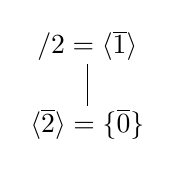
\begin{tikzpicture}[baseline=(current bounding box.center), every node/.style={inner sep=1pt}]
					\node (a) at (0,0.8) {$\ZZ/2\ZZ=\langle \overline{1}\rangle$};
					\node (b) at (0,-0.2) {$\langle\overline{2}\rangle=\{\overline{0}\}$};
					\draw (a)--(b);
				\end{tikzpicture}
			\end{minipage}
			\begin{minipage}{0.42\linewidth}
				\centering
				\begin{tikzpicture}[baseline=(current bounding box.center), every node/.style={inner sep=1pt}]
					\node (a) at (0,1.2) {$\ZZ/4\ZZ=\langle \overline{1}\rangle$};
					\node (note) at (2.5,1.2) {\small（注意：$\langle\overline{1}\rangle=\langle\overline{3}\rangle$）};
					\node (b) at (0,0.1) {$\langle\overline{2}\rangle$};
					\node (c) at (0,-1.0) {$\langle\overline{4}\rangle=\{\overline{0}\}$};
					\draw (a)--(b)--(c);
				\end{tikzpicture}
			\end{minipage}
		\end{center}
		
		\begin{center}
			\begin{tikzpicture}[every node/.style={inner sep=1pt}]
				\node (a) at (0,1.8) {$\ZZ/8\ZZ=\langle\overline{1}\rangle$};
				\node (note) at (3.8,1.8) {\small（注意：$\langle\overline{1}\rangle=\langle\overline{3}\rangle=\langle\overline{5}\rangle=\langle\overline{7}\rangle$）};
				\node (b) at (0,0.7) {$\langle\overline{2}\rangle$};
				\node (c) at (0,-0.4) {$\langle\overline{4}\rangle$};
				\node (d) at (0,-1.5) {$\langle\overline{8}\rangle=\{\overline{0}\}$};
				\draw (a)--(b)--(c)--(d);
			\end{tikzpicture}
		\end{center}
		
		一般地，若 $p$ 是素数，则 $\ZZ/p^n\ZZ$ 的格为
		\begin{center}
			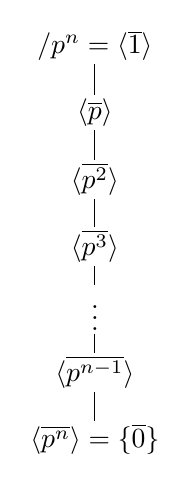
\begin{tikzpicture}[every node/.style={inner sep=1pt}]
				\node (a) at (0,2.8) {$\ZZ/p^n\ZZ=\langle\overline{1}\rangle$};
				\node (b) at (0,1.95) {$\langle\overline{p}\rangle$};
				\node (c) at (0,1.1) {$\langle\overline{p^2}\rangle$};
				\node (d) at (0,0.25) {$\langle\overline{p^3}\rangle$};
				\node (e) at (0,-0.55) {$\vdots$};
				\node (f) at (0,-1.35) {$\langle\overline{p^{n-1}}\rangle$};
				\node (g) at (0,-2.2) {$\langle\overline{p^n}\rangle=\{\overline{0}\}$};
				\draw (a)--(b)--(c)--(d)--(e)--(f)--(g);
			\end{tikzpicture}
		\end{center}
		
		\begin{center}
			\begin{minipage}{0.45\linewidth}
				\centering
				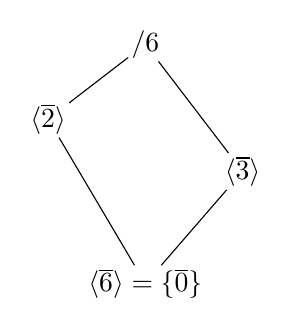
\begin{tikzpicture}[scale=.95, every node/.style={inner sep=1pt}]
					\node (top) at (0,2) {$\ZZ/6\ZZ$};
					\node (a) at (-1.3,1) {$\langle\overline{2}\rangle$};
					\node (b) at (1.3,0.3) {$\langle\overline{3}\rangle$};
					\node (bot) at (0,-1.2) {$\langle\overline{6}\rangle=\{\overline{0}\}$};
					\draw (top)--(a)--(bot)--(b)--(top);
				\end{tikzpicture}
			\end{minipage}
			\begin{minipage}{0.45\linewidth}
				\centering
				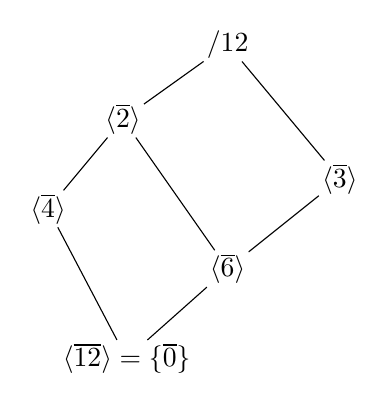
\begin{tikzpicture}[scale=.95, every node/.style={inner sep=1pt}]
					\node (top) at (0,2.2) {$\ZZ/12\ZZ$};
					\node (a) at (-1.4,1.2) {$\langle\overline{2}\rangle$};
					\node (b) at (1.5,.4) {$\langle\overline{3}\rangle$};
					\node (c) at (-2.4,0) {$\langle\overline{4}\rangle$};
					\node (d) at (0,-.8) {$\langle\overline{6}\rangle$};
					\node (bot) at (-1.35,-2.0) {$\langle\overline{12}\rangle=\{\overline{0}\}$};
					\draw (top)--(a)--(c)--(bot)--(d)--(b)--(top);
					\draw (a)--(d);
				\end{tikzpicture}
			\end{minipage}
		\end{center}
		\item \textbf{克莱因四元群}（Viergruppe）$V_4$ 是阶为 $4$ 的群，其乘法表与格为
		\begin{center}
			\begin{tabular}{c@{\qquad}c}
				$\begin{array}{c|cccc}
					\cdot&1&a&b&c\\ \hline
					1&1&a&b&c\\
					a&a&1&c&b\\
					b&b&c&1&a\\
					c&c&b&a&1
				\end{array}$
				&
				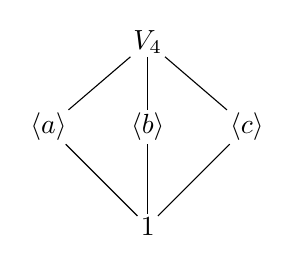
\begin{tikzpicture}[baseline=(current bounding box.center), scale=.9, every node/.style={inner sep=1pt}]
					\node (top) at (0,2) {$V_4$};
					\node (a) at (-1.4,.8) {$\langle a\rangle$};
					\node (b) at (0,.8) {$\langle b\rangle$};
					\node (c) at (1.4,.8) {$\langle c\rangle$};
					\node (bot) at (0,-.6) {$1$};
					\draw (top)--(a)--(bot)--(c)--(top);
					\draw (top)--(b)--(bot);
				\end{tikzpicture}
			\end{tabular}
		\end{center}
		注意 $V_4$ 是阿贝尔群，且不同构于 $Z_4$。我们会看到 $D_8$ 含有一个同构于 $V_4$ 的子群，因此不必检查上述定义的二元运算满足结合律。
		
		\item $S_3$ 的格为
		\begin{center}
			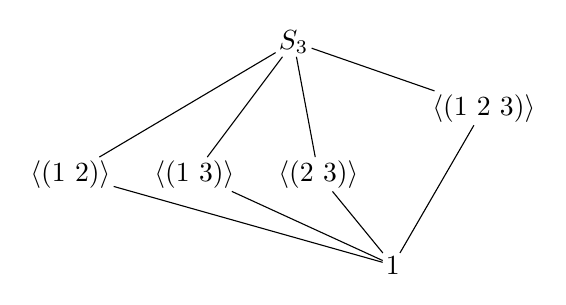
\begin{tikzpicture}[scale=1.05, every node/.style={inner sep=1pt}]
				\node (top) at (0,2.2) {$S_3$};
				\node (a) at (-2.7,.6) {$\langle(1\ 2)\rangle$};
				\node (b) at (-1.2,.6) {$\langle(1\ 3)\rangle$};
				\node (c) at (.3,.6) {$\langle(2\ 3)\rangle$};
				\node (d) at (2.3,1.4) {$\langle(1\ 2\ 3)\rangle$};
				\node (bot) at (1.2,-.5) {$1$};
				\foreach \x in {a,b,c,d} {\draw (top)--(\x); \draw (\x)--(bot);}
			\end{tikzpicture}
		\end{center}
		
		\item 用通常记号 $D_8=\langle r,s\rangle$，$D_8$ 的格为
		\begin{center}
		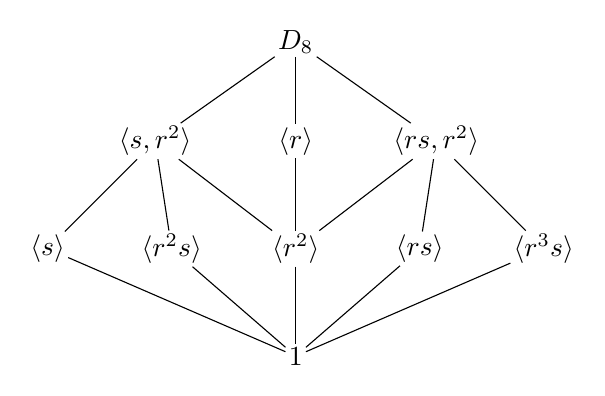
\begin{tikzpicture}[scale=1.05, every node/.style={inner sep=1pt}]
			\node (top) at (0,3) {$D_8$};
			\node (a) at (-1.7,1.8) {$\langle s,r^2\rangle$};
			\node (b) at (0,1.8) {$\langle r\rangle$};
			\node (c) at (1.7,1.8) {$\langle rs,r^2\rangle$};
			\node (d) at (-3,.5) {$\langle s\rangle$};
			\node (e) at (-1.5,.5) {$\langle r^2s\rangle$};
			\node (f) at (0,.5) {$\langle r^2\rangle$};
			\node (g) at (1.5,.5) {$\langle rs\rangle$};
			\node (h) at (3,.5) {$\langle r^3s\rangle$};
			\node (bot) at (0,-.8) {$1$};
			\draw (top)--(a)--(d)--(bot);
			\draw (top)--(b)--(f)--(bot);
			\draw (top)--(c)--(h)--(bot);
			\draw (a)--(e)--(bot);
			\draw (a)--(f);
			\draw (c)--(f);
			\draw (c)--(g)--(bot);
		\end{tikzpicture}
		\end{center}
		\item $D_{16}$ 的子群格不是平面图（不能在平面上画出而不使线相交）。它的一种画法是
		\begin{center}
			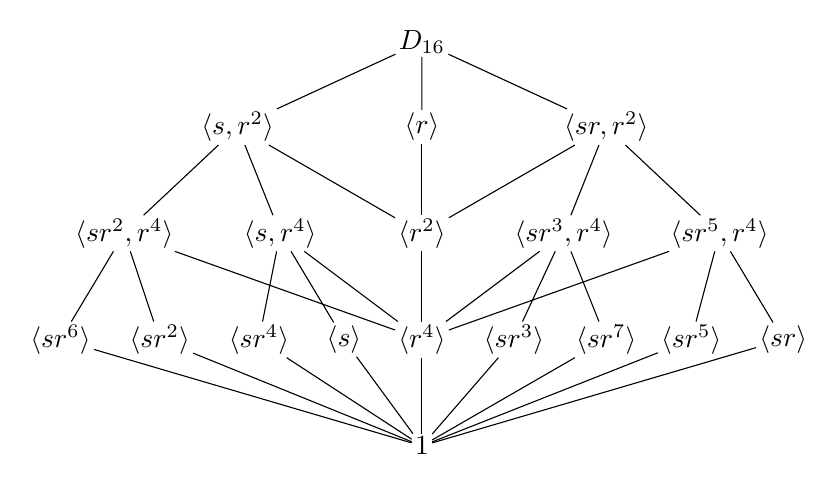
\begin{tikzpicture}[scale=.9, every node/.style={inner sep=1pt}]
				\node (top) at (0,5) {$D_{16}$};
				\node (sr2) at (-2.6,3.8) {$\langle s,r^2\rangle$};
				\node (r) at (0,3.8) {$\langle r\rangle$};
				\node (srr2) at (2.6,3.8) {$\langle sr,r^2\rangle$};
				\node (sr2r4) at (-4.2,2.3) {$\langle sr^2,r^4\rangle$};
				\node (sr4) at (-2,2.3) {$\langle s,r^4\rangle$};
				\node (r2) at (0,2.3) {$\langle r^2\rangle$};
				\node (sr3r4) at (2,2.3) {$\langle sr^3,r^4\rangle$};
				\node (sr5r4) at (4.2,2.3) {$\langle sr^5,r^4\rangle$};
				\node (sr6) at (-5.1,.8) {$\langle sr^6\rangle$};
				\node (sr2s) at (-3.7,.8) {$\langle sr^2\rangle$};
				\node (sr4s) at (-2.3,.8) {$\langle sr^4\rangle$};
				\node (ss) at (-1.1,.8) {$\langle s\rangle$};
				\node (r4) at (0,.8) {$\langle r^4\rangle$};
				\node (sr3) at (1.3,.8) {$\langle sr^3\rangle$};
				\node (sr7) at (2.6,.8) {$\langle sr^7\rangle$};
				\node (sr5) at (3.8,.8) {$\langle sr^5\rangle$};
				\node (sr) at (5.1,.8) {$\langle sr\rangle$};
				\node (bot) at (0,-.7) {$1$};
				\draw (top)--(sr2) (top)--(r) (top)--(srr2);
				\draw (sr2)--(sr2r4) (sr2)--(sr4) (sr2)--(r2);
				\draw (r)--(r2);
				\draw (srr2)--(r2) (srr2)--(sr3r4) (srr2)--(sr5r4);
				\draw (sr2r4)--(sr6) (sr2r4)--(sr2s) (sr2r4)--(r4);
				\draw (sr4)--(sr4s) (sr4)--(ss) (sr4)--(r4);
				\draw (r2)--(r4);
				\draw (sr3r4)--(r4) (sr3r4)--(sr3) (sr3r4)--(sr7);
				\draw (sr5r4)--(r4) (sr5r4)--(sr5) (sr5r4)--(sr);
				\foreach \x in {sr6,sr2s,sr4s,ss,r4,sr3,sr7,sr5,sr} {\draw (\x)--(bot);}
			\end{tikzpicture}
		\end{center}
	\end{enumerate}
	
	
\end{example}


在理论证明和具体例子中，我们常常只关心给定群的两个（或少数几个）子群及其相互关系。为了把这些关系画出来，我们将画出整个群格的一个\textbf{子格}，其中包含相关的上确界与交。这样的子格中的一条不断开的线一般并不表示该线两端之间没有其他子群。这些部分格也会在处理无限群时使用。例如，若只想讨论 $D_{16}$ 的子群 $\langle sr^2,r^4\rangle$ 与 $\langle r^2\rangle$ 的关系，可画出如下子格：
\begin{center}
	\begin{tikzpicture}[scale=1.0, every node/.style={inner sep=1pt}]
		\node (top) at (0,4) {$D_{16}$};
		\node (a) at (0,3) {$\langle s,r^2\rangle$};
		\node (b) at (-1.5,1.8) {$\langle sr^2,r^4\rangle$};
		\node (c) at (1.5,1.8) {$\langle r^2\rangle$};
		\node (d) at (0,.6) {$\langle r^4\rangle$};
		\node (bot) at (0,-.5) {$1$};
		\draw (top)--(a)--(b)--(d)--(bot);
		\draw (a)--(c)--(d);
	\end{tikzpicture}
\end{center}
注意 $\langle s,r^2\rangle$ 和 $\langle r^4\rangle$ 分别正是这两个子群在 $D_{16}$ 中的上确界与交。

最后，给定一个群的子群格后，计算正规化子和中心化子相对容易。例如，在 $D_8$ 中，可以看出 $C_{D_8}(s)=\langle s,r^2\rangle$，因为先计算得 $r^2\in C_{D_8}(s)$（见第 2 节）。这证明 $\langle s,r^2\rangle\leq C_{D_8}(s)$（注意一个元素总属于它自身的中心化子）。包含 $\langle s,r^2\rangle$ 的子群只有它自身和整个 $D_8$。不可能有 $C_{D_8}(s)=D_8$，因为 $r$ 不与 $s$ 交换（即 $r\notin C_{D_8}(s)$）。于是只剩所声称的一种可能。


